\documentclass[11pt,twocolumn]{article}
\usepackage{lmodern}
\usepackage[backend=biber, style=ieee]{biblatex}
\usepackage{easylist}
\usepackage{hanging}
\usepackage{hyperref}
\usepackage{blindtext}
\usepackage{tipa}
\usepackage[left=2.5cm, top=2cm, bottom=2cm, right=2.5cm]{geometry}
\begin{document}
\textbf{AIM:} Addition of two 8 bit numbers and

\begin{enumerate}
\def\labelenumi{\arabic{enumi}.}
\item
  Sum is also 8 bit number
\item
  Sum is 16 bit number
\end{enumerate}

\textbf{{[}SOFTWARE USED{]} :} GNUSim 8085

\textbf{{[}THEORY{]}:}

The Intel 8085 is an 8-bit microprocessor produced by Intel and
introduced in March 1976. It is a software-binary compatible with the
more-famous Intel 8080 with only two minor instructions added to support
its added interrupt and serial input/output features.

\textbf{INSTRUCTIONS IN 8085:}

An instruction of a computer is a command given to the computer to
perform a specified operation on given data. In microprocessor, the
instruction set is the collection of the instructions that the
microprocessor is designed to execute.

The programmer writes a program in assembly language using these
instructions. These instructions have been classified into the following
groups:

\begin{enumerate}
\def\labelenumi{\arabic{enumi}.}
\item
  \textbf{Data Transfer Group}
\item
  \textbf{Arithmetic Group}
\item
  \textbf{Logical Group}
\item
  \textbf{Branch Control Group}
\item
  \textbf{I/O and Machine Control Group}
\end{enumerate}

These are briefly explained below

\begin{enumerate}
\def\labelenumi{\arabic{enumi}.}
\tightlist
\item
  \textbf{Data Transfer Group}
\end{enumerate}

Instructions, which are used to transfer data from one register to
another register, from memory to register or register to memory, come
under this group. Examples are: MOV, MVI, LXI, LDA, STA etc. When an
instruction of data transfer group is executed, data is transferred from
the source to the destination without altering the contents of the
source

\begin{enumerate}
\def\labelenumi{\arabic{enumi}.}
\setcounter{enumi}{1}
\tightlist
\item
  \textbf{Arithmetic Group}
\end{enumerate}

The instructions of this group perform arithmetic operations such as
addition, subtraction; increment or decrement of the content of a
register or memory. Examples are: ADD, SUB, INR, DAD etc\textbf{.}

\begin{enumerate}
\def\labelenumi{\arabic{enumi}.}
\setcounter{enumi}{2}
\tightlist
\item
  \textbf{Logical Group}
\end{enumerate}

The Instructions under this group perform logical operation such as AND,
OR, compare, rotate etc. Examples are: ANA, XRA, ORA, CMP, and RAL etc.

\begin{enumerate}
\def\labelenumi{\arabic{enumi}.}
\setcounter{enumi}{3}
\tightlist
\item
  \textbf{Branch Control Group}
\end{enumerate}

This group includes the instructions for conditional and unconditional
jump, subroutine call and return, and restart. Examples are: JMP, JC,
JZ, CALL, CZ, RST etc.

\begin{enumerate}
\def\labelenumi{\arabic{enumi}.}
\setcounter{enumi}{4}
\tightlist
\item
  \textbf{I/O and Machine Control Group}
\end{enumerate}

This group includes the instructions for input/output ports, stack and
machine

control. Examples are: IN, OUT, PUSH, POP, and HLT etc

\textbf{{[}ALGORITHM{]}}

\begin{enumerate}
\def\labelenumi{\alph{enumi})}
\tightlist
\item
  {[}Sum is 8 bit{]}
\end{enumerate}

\begin{itemize}
\item
  Get address of first number in H-L pair
\item
  First number in accumulator
\item
  Increment content of H-L pair
\item
  Add first and second number
\item
  Store sum in 2503 H
\item
  Stop
\end{itemize}

\begin{enumerate}
\def\labelenumi{\alph{enumi})}
\setcounter{enumi}{1}
\tightlist
\item
  {[}Sum is 16 bit{]}
\end{enumerate}

\begin{itemize}
\item
  Address of first number in H-L pair
\item
  MSBs of sum in in register C. Initial value=00
\item
  First number in accumulator
\item
  Address of Second number in H-L pair
\item
  Add the two numbers
\item
  Is carry? If no, go to label AHEAD
\item
  If yes, increment C
\item
  LSB of sum in 2503 H
\item
  MSB of sum in accumulator
\item
  MSB of sum in 2504 H
\item
  Stop
\end{itemize}

\textbf{{[}FLOW CHART{]}:}

\begin{enumerate}
\def\labelenumi{\alph{enumi})}
\tightlist
\item
  Sum is 8 bit
\end{enumerate}

\begin{verbatim}
graph TB
st([Start]) --> op1[Load H-L pair with first operands memory address]

op1 --> op2[Move the first operand from memory to accumulator]
op2 --> op3[Increament H-L pair to point next memory location]
op3 --> op4[Add with A]
op4 --> op5[Increment H-L pair]
op5 --> op6[Move the result from accumulator to memory]
op6 --> Stop
\end{verbatim}

\begin{enumerate}
\def\labelenumi{\alph{enumi})}
\setcounter{enumi}{1}
\tightlist
\item
  {[}Sum is 16 bit{]}
\end{enumerate}

\begin{verbatim}
graph TB
st[Start]-->op1[Load H-L pair with first operands memory address]
op1 --> op2[move the first operand from memory to accumulator]
op2 --> op3[Increament H-L pair to point next memory location]
op3 --> op4[Initialize register  C = 00]
op4 -->op5[Add M with A]
op5 --> cond{If Carry ?}
cond -->|yes|op6[Increment register C]
op6 -->op7[Increment H-L pairt]
op7 -->op8[Move the result to memory]
op8 -->op9[Increment H-L pair and move carry from register C to memory]
op9 --> Stop

cond -->|no|op7
\end{verbatim}

\begin{center}\rule{0.5\linewidth}{0.5pt}\end{center}

\begin{verbatim}
st=>start: Start
e=>end: Stop
op1=>operation: Load H-L pair with first operands memory address
op2=>operation: move the first operand from memory to accumulator
op3=>operation: Increament H-L pair to point next memory location
op4=>operation: Add with A
op5=>operation: Increment H-L pair
op6=>operation: Move the result from accumulator to memory

st->op1->op2->op3->op4->op5->op6->e
\end{verbatim}

\begin{enumerate}
\def\labelenumi{\alph{enumi})}
\setcounter{enumi}{1}
\tightlist
\item
  {[}Sum is 16 bit{]}
\end{enumerate}

\begin{verbatim}
st=>start: Start
e=>end: Stop
op1=>operation: Load H-L pair with first operands memory address
op2=>operation: move the first operand from memory to accumulator
op3=>operation: Increament H-L pair to point next memory location
op4=>operation: Initialize register  C = 00
op5=>operation: Add M with A
cond=>condition: if carry ?
op6=>operation: Increment register C
op7=>operation: Increment H-L pairt
op8=>operation: Move the result to memory
op9=>operation: Increment H-L pair and move carry from register C to memory


st->op1->op2->op3->op4->op5->cond
cond(yes)->op6->op7->op8->op9->e
cond(no)-

op6[Increment register C]
op7[Increment H-L pairt]
op8[Move the result to memory]
op9[Increment H-L pair and move carry from register C to memory]
\end{verbatim}

\textbf{{[}PROGRAM AND OUTPUT{]}:}

\begin{enumerate}
\def\labelenumi{\alph{enumi})}
\tightlist
\item
  {[}Sum is 8 bit{]}
\end{enumerate}

\begin{longtable}[]{@{}lllllll@{}}
\toprule
\begin{minipage}[b]{0.04\columnwidth}\raggedright
Add\strut
\end{minipage} & \begin{minipage}[b]{0.05\columnwidth}\raggedright
Mnemo\strut
\end{minipage} & \begin{minipage}[b]{0.05\columnwidth}\raggedright
Op\strut
\end{minipage} & \begin{minipage}[b]{0.37\columnwidth}\raggedright
Comments\strut
\end{minipage} & \begin{minipage}[b]{0.09\columnwidth}\raggedright
Addressing Mode\strut
\end{minipage} & \begin{minipage}[b]{0.17\columnwidth}\raggedright
Machine Cycle\strut
\end{minipage} & \begin{minipage}[b]{0.05\columnwidth}\raggedright
T-States\strut
\end{minipage}\tabularnewline
\midrule
\endhead
\begin{minipage}[t]{0.04\columnwidth}\raggedright
2000\strut
\end{minipage} & \begin{minipage}[t]{0.05\columnwidth}\raggedright
LXI H\strut
\end{minipage} & \begin{minipage}[t]{0.05\columnwidth}\raggedright
2501H\strut
\end{minipage} & \begin{minipage}[t]{0.37\columnwidth}\raggedright
Load H-L pairs with address 2501H\strut
\end{minipage} & \begin{minipage}[t]{0.09\columnwidth}\raggedright
Immediate\strut
\end{minipage} & \begin{minipage}[t]{0.17\columnwidth}\raggedright
Opcode fetch + 2 Memory read\strut
\end{minipage} & \begin{minipage}[t]{0.05\columnwidth}\raggedright
10\strut
\end{minipage}\tabularnewline
\begin{minipage}[t]{0.04\columnwidth}\raggedright
2003\strut
\end{minipage} & \begin{minipage}[t]{0.05\columnwidth}\raggedright
MOV A, M\strut
\end{minipage} & \begin{minipage}[t]{0.05\columnwidth}\raggedright
\strut
\end{minipage} & \begin{minipage}[t]{0.37\columnwidth}\raggedright
Move first operand from memory to accumulator\strut
\end{minipage} & \begin{minipage}[t]{0.09\columnwidth}\raggedright
Indirect\strut
\end{minipage} & \begin{minipage}[t]{0.17\columnwidth}\raggedright
Opcode fetch + Memory read\strut
\end{minipage} & \begin{minipage}[t]{0.05\columnwidth}\raggedright
7\strut
\end{minipage}\tabularnewline
\begin{minipage}[t]{0.04\columnwidth}\raggedright
2004\strut
\end{minipage} & \begin{minipage}[t]{0.05\columnwidth}\raggedright
INX H\strut
\end{minipage} & \begin{minipage}[t]{0.05\columnwidth}\raggedright
\strut
\end{minipage} & \begin{minipage}[t]{0.37\columnwidth}\raggedright
Increment H-L pair\strut
\end{minipage} & \begin{minipage}[t]{0.09\columnwidth}\raggedright
Register\strut
\end{minipage} & \begin{minipage}[t]{0.17\columnwidth}\raggedright
Opcode fetch\strut
\end{minipage} & \begin{minipage}[t]{0.05\columnwidth}\raggedright
6\strut
\end{minipage}\tabularnewline
\begin{minipage}[t]{0.04\columnwidth}\raggedright
2005\strut
\end{minipage} & \begin{minipage}[t]{0.05\columnwidth}\raggedright
ADD M\strut
\end{minipage} & \begin{minipage}[t]{0.05\columnwidth}\raggedright
\strut
\end{minipage} & \begin{minipage}[t]{0.37\columnwidth}\raggedright
Add M with A\strut
\end{minipage} & \begin{minipage}[t]{0.09\columnwidth}\raggedright
Register\strut
\end{minipage} & \begin{minipage}[t]{0.17\columnwidth}\raggedright
Opcode fetch + Memory read\strut
\end{minipage} & \begin{minipage}[t]{0.05\columnwidth}\raggedright
7\strut
\end{minipage}\tabularnewline
\begin{minipage}[t]{0.04\columnwidth}\raggedright
2006\strut
\end{minipage} & \begin{minipage}[t]{0.05\columnwidth}\raggedright
INX H\strut
\end{minipage} & \begin{minipage}[t]{0.05\columnwidth}\raggedright
\strut
\end{minipage} & \begin{minipage}[t]{0.37\columnwidth}\raggedright
Increment H-L pair\strut
\end{minipage} & \begin{minipage}[t]{0.09\columnwidth}\raggedright
Register\strut
\end{minipage} & \begin{minipage}[t]{0.17\columnwidth}\raggedright
Opcode fetch\strut
\end{minipage} & \begin{minipage}[t]{0.05\columnwidth}\raggedright
6\strut
\end{minipage}\tabularnewline
\begin{minipage}[t]{0.04\columnwidth}\raggedright
2007\strut
\end{minipage} & \begin{minipage}[t]{0.05\columnwidth}\raggedright
MOV M, A\strut
\end{minipage} & \begin{minipage}[t]{0.05\columnwidth}\raggedright
\strut
\end{minipage} & \begin{minipage}[t]{0.37\columnwidth}\raggedright
Move contents of Accumulator to memory add sotred in H-L Pair\strut
\end{minipage} & \begin{minipage}[t]{0.09\columnwidth}\raggedright
Indirect\strut
\end{minipage} & \begin{minipage}[t]{0.17\columnwidth}\raggedright
Opcode fetch + memory write\strut
\end{minipage} & \begin{minipage}[t]{0.05\columnwidth}\raggedright
7\strut
\end{minipage}\tabularnewline
\begin{minipage}[t]{0.04\columnwidth}\raggedright
2008\strut
\end{minipage} & \begin{minipage}[t]{0.05\columnwidth}\raggedright
HLT\strut
\end{minipage} & \begin{minipage}[t]{0.05\columnwidth}\raggedright
\strut
\end{minipage} & \begin{minipage}[t]{0.37\columnwidth}\raggedright
HALT\strut
\end{minipage} & \begin{minipage}[t]{0.09\columnwidth}\raggedright
-\strut
\end{minipage} & \begin{minipage}[t]{0.17\columnwidth}\raggedright
Opcode fetch\strut
\end{minipage} & \begin{minipage}[t]{0.05\columnwidth}\raggedright
4\strut
\end{minipage}\tabularnewline
\bottomrule
\end{longtable}

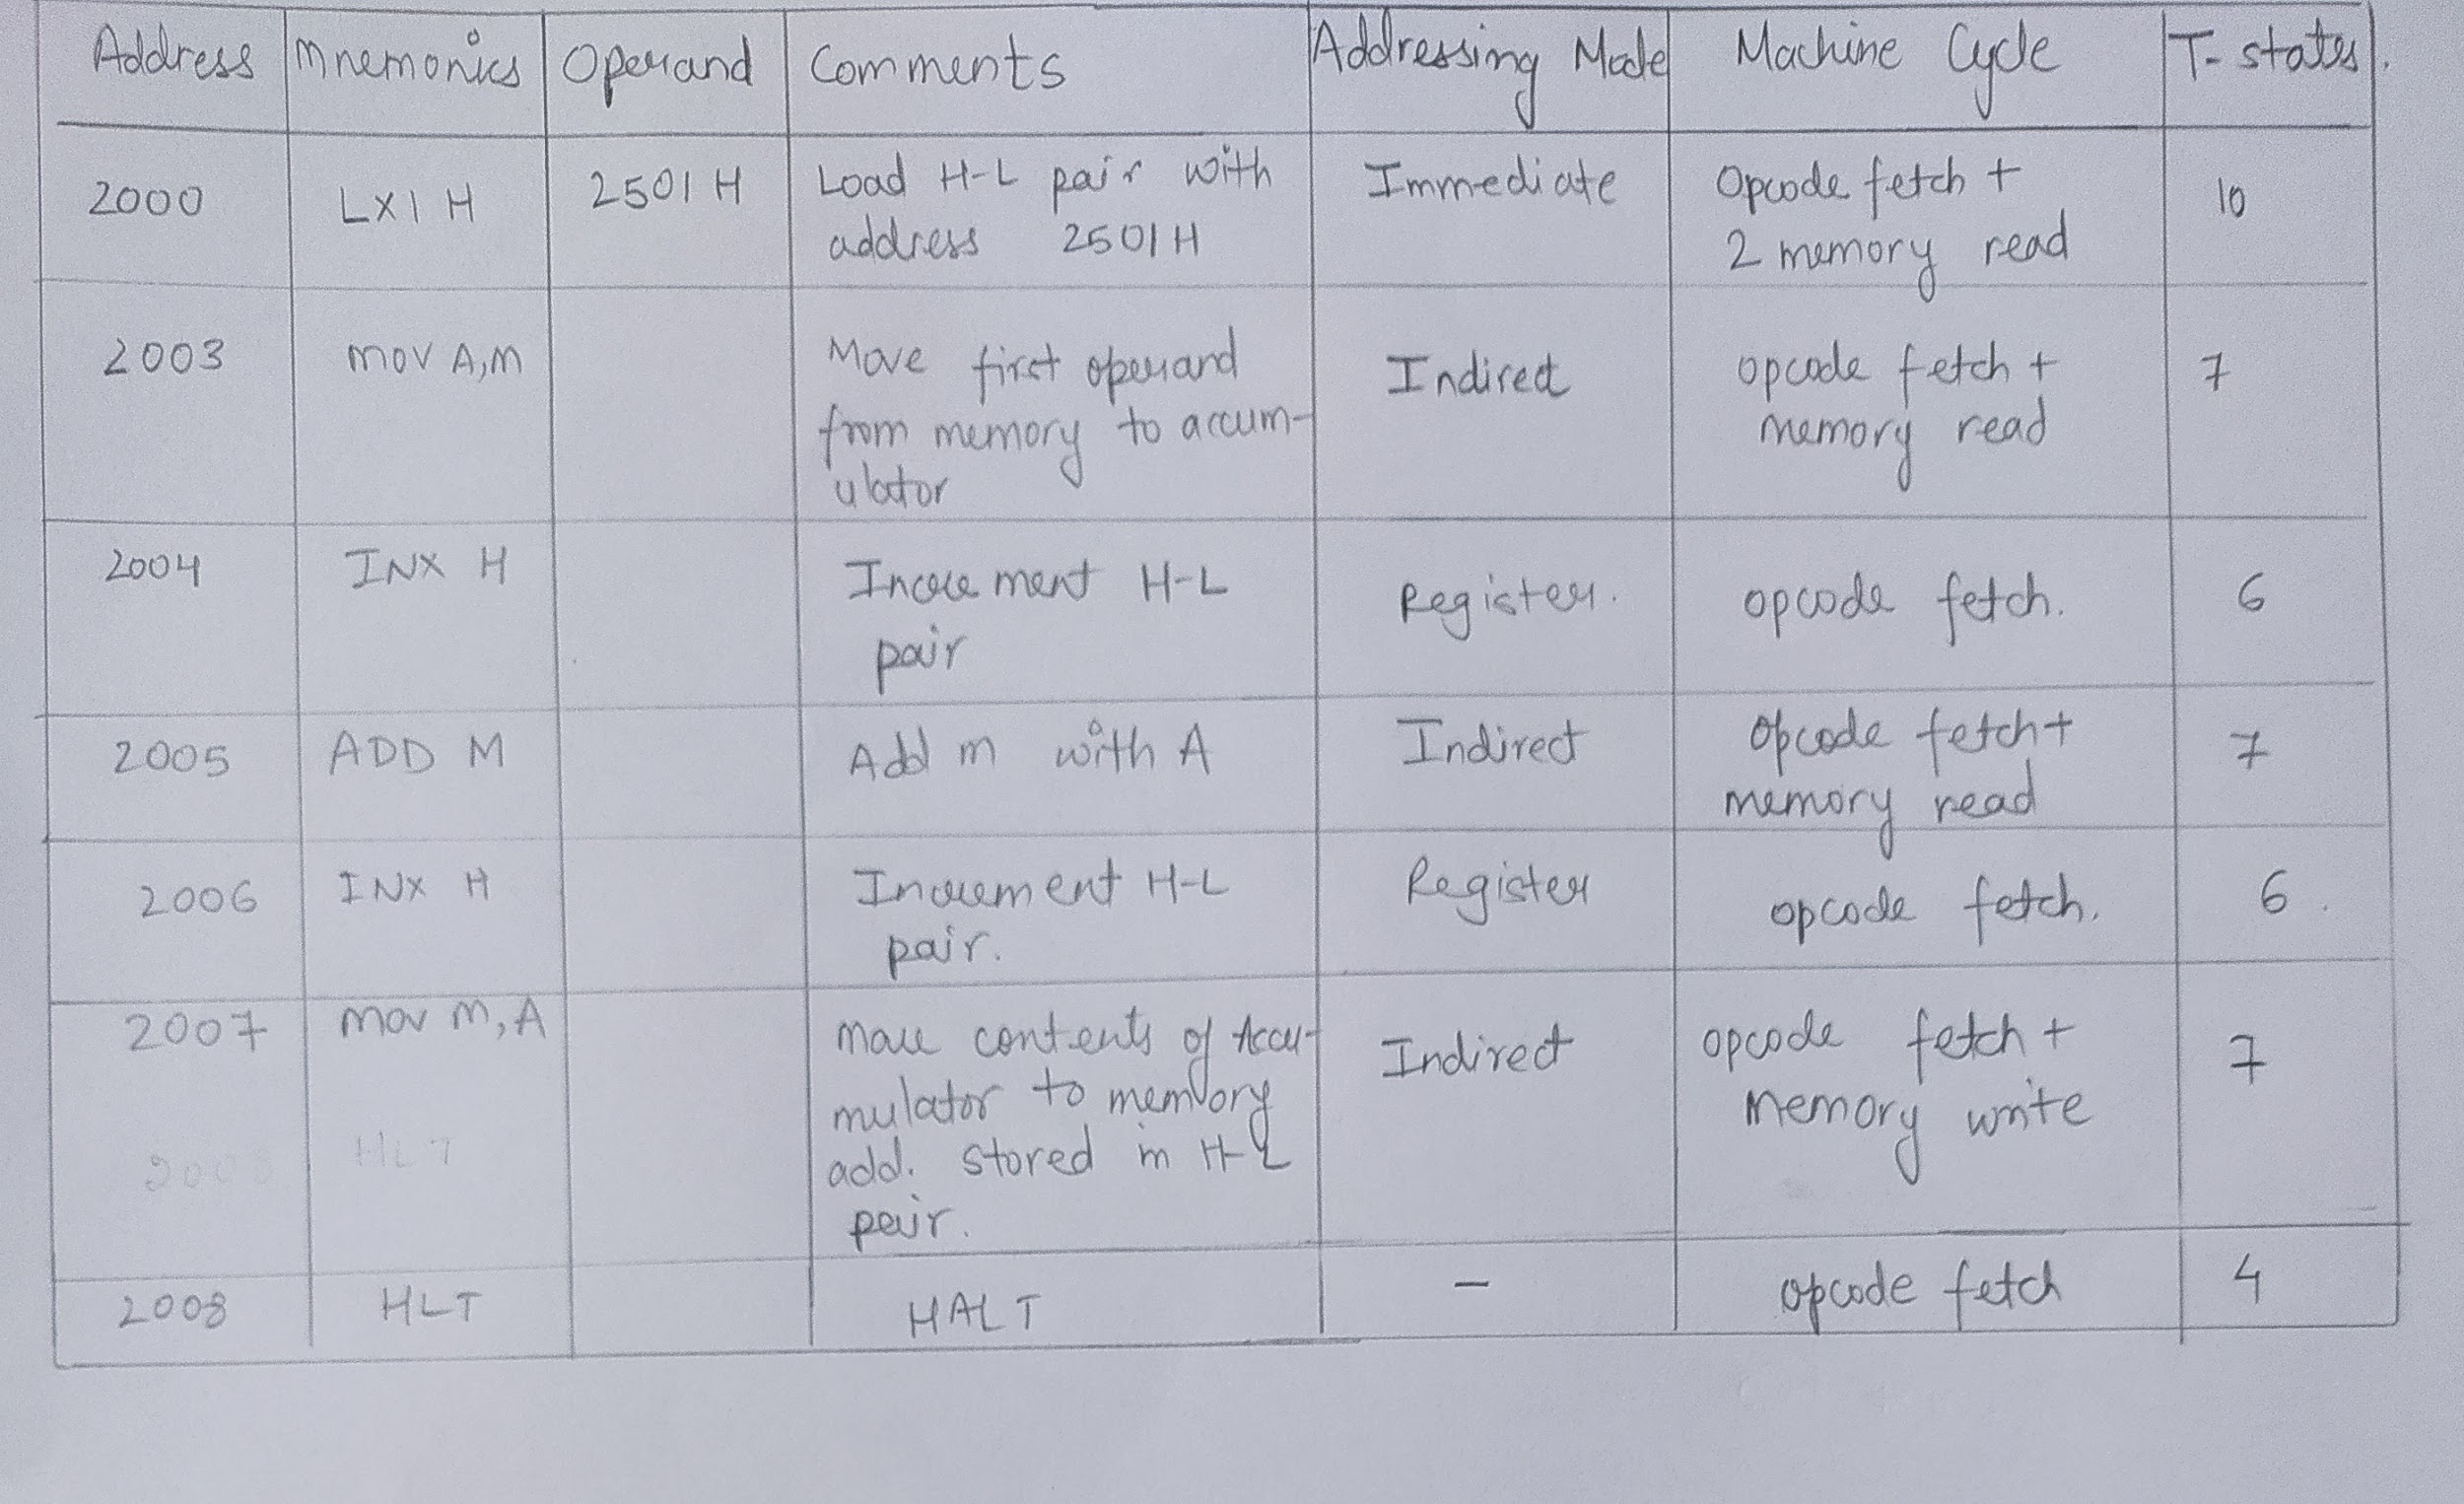
\includegraphics[width=6.35in,height=3.87727in]{media/image1.jpg}

\textbf{{[}Output:{]}}

2501- 04 H

2502- 02 H

2503- 06 H

\pagebreak

\begin{enumerate}
\def\labelenumi{\alph{enumi})}
\setcounter{enumi}{1}
\tightlist
\item
  {[}Sum is 16 bit{]}
\end{enumerate}

\begin{longtable}[]{@{}llllllll@{}}
\toprule
\begin{minipage}[b]{0.04\columnwidth}\raggedright
Add\strut
\end{minipage} & \begin{minipage}[b]{0.05\columnwidth}\raggedright
Mn\strut
\end{minipage} & \begin{minipage}[b]{0.05\columnwidth}\raggedright
Op\strut
\end{minipage} & \begin{minipage}[b]{0.23\columnwidth}\raggedright
Comments\strut
\end{minipage} & \begin{minipage}[b]{0.09\columnwidth}\raggedright
Addressing Mode\strut
\end{minipage} & \begin{minipage}[b]{0.25\columnwidth}\raggedright
Machine Cycle\strut
\end{minipage} & \begin{minipage}[b]{0.05\columnwidth}\raggedright
T-States\strut
\end{minipage} & \begin{minipage}[b]{0.03\columnwidth}\raggedright
Lable\strut
\end{minipage}\tabularnewline
\midrule
\endhead
\begin{minipage}[t]{0.04\columnwidth}\raggedright
2000\strut
\end{minipage} & \begin{minipage}[t]{0.05\columnwidth}\raggedright
LXI H\strut
\end{minipage} & \begin{minipage}[t]{0.05\columnwidth}\raggedright
2501 H\strut
\end{minipage} & \begin{minipage}[t]{0.23\columnwidth}\raggedright
Load H-L pair with Address 300H\strut
\end{minipage} & \begin{minipage}[t]{0.09\columnwidth}\raggedright
Immediate\strut
\end{minipage} & \begin{minipage}[t]{0.25\columnwidth}\raggedright
Opcode fetch and 2 memory read\strut
\end{minipage} & \begin{minipage}[t]{0.05\columnwidth}\raggedright
10\strut
\end{minipage} & \begin{minipage}[t]{0.03\columnwidth}\raggedright
\strut
\end{minipage}\tabularnewline
\begin{minipage}[t]{0.04\columnwidth}\raggedright
2003\strut
\end{minipage} & \begin{minipage}[t]{0.05\columnwidth}\raggedright
MVI C\strut
\end{minipage} & \begin{minipage}[t]{0.05\columnwidth}\raggedright
00\strut
\end{minipage} & \begin{minipage}[t]{0.23\columnwidth}\raggedright
Initialize C register with zero value\strut
\end{minipage} & \begin{minipage}[t]{0.09\columnwidth}\raggedright
Immediate\strut
\end{minipage} & \begin{minipage}[t]{0.25\columnwidth}\raggedright
Opcode fetch + memory read\strut
\end{minipage} & \begin{minipage}[t]{0.05\columnwidth}\raggedright
7\strut
\end{minipage} & \begin{minipage}[t]{0.03\columnwidth}\raggedright
\strut
\end{minipage}\tabularnewline
\begin{minipage}[t]{0.04\columnwidth}\raggedright
2005\strut
\end{minipage} & \begin{minipage}[t]{0.05\columnwidth}\raggedright
MOV A, M\strut
\end{minipage} & \begin{minipage}[t]{0.05\columnwidth}\raggedright
\strut
\end{minipage} & \begin{minipage}[t]{0.23\columnwidth}\raggedright
Move first operand form memory to A\strut
\end{minipage} & \begin{minipage}[t]{0.09\columnwidth}\raggedright
Indirect\strut
\end{minipage} & \begin{minipage}[t]{0.25\columnwidth}\raggedright
Opcode fetch + memory read\strut
\end{minipage} & \begin{minipage}[t]{0.05\columnwidth}\raggedright
7\strut
\end{minipage} & \begin{minipage}[t]{0.03\columnwidth}\raggedright
\strut
\end{minipage}\tabularnewline
\begin{minipage}[t]{0.04\columnwidth}\raggedright
2006\strut
\end{minipage} & \begin{minipage}[t]{0.05\columnwidth}\raggedright
INX H\strut
\end{minipage} & \begin{minipage}[t]{0.05\columnwidth}\raggedright
\strut
\end{minipage} & \begin{minipage}[t]{0.23\columnwidth}\raggedright
Increment H-L Pair\strut
\end{minipage} & \begin{minipage}[t]{0.09\columnwidth}\raggedright
Register\strut
\end{minipage} & \begin{minipage}[t]{0.25\columnwidth}\raggedright
Opcode fetch\strut
\end{minipage} & \begin{minipage}[t]{0.05\columnwidth}\raggedright
6\strut
\end{minipage} & \begin{minipage}[t]{0.03\columnwidth}\raggedright
\strut
\end{minipage}\tabularnewline
\begin{minipage}[t]{0.04\columnwidth}\raggedright
2007\strut
\end{minipage} & \begin{minipage}[t]{0.05\columnwidth}\raggedright
ADD M\strut
\end{minipage} & \begin{minipage}[t]{0.05\columnwidth}\raggedright
\strut
\end{minipage} & \begin{minipage}[t]{0.23\columnwidth}\raggedright
Add M with A\strut
\end{minipage} & \begin{minipage}[t]{0.09\columnwidth}\raggedright
Indirect\strut
\end{minipage} & \begin{minipage}[t]{0.25\columnwidth}\raggedright
Opcode fetch + memory read\strut
\end{minipage} & \begin{minipage}[t]{0.05\columnwidth}\raggedright
7\strut
\end{minipage} & \begin{minipage}[t]{0.03\columnwidth}\raggedright
\strut
\end{minipage}\tabularnewline
\begin{minipage}[t]{0.04\columnwidth}\raggedright
2008\strut
\end{minipage} & \begin{minipage}[t]{0.05\columnwidth}\raggedright
JNC\strut
\end{minipage} & \begin{minipage}[t]{0.05\columnwidth}\raggedright
AHEAD\strut
\end{minipage} & \begin{minipage}[t]{0.23\columnwidth}\raggedright
Jump to label if no carry\strut
\end{minipage} & \begin{minipage}[t]{0.09\columnwidth}\raggedright
Immediate\strut
\end{minipage} & \begin{minipage}[t]{0.25\columnwidth}\raggedright
Opcode fetch + 2 memory read\strut
\end{minipage} & \begin{minipage}[t]{0.05\columnwidth}\raggedright
10\strut
\end{minipage} & \begin{minipage}[t]{0.03\columnwidth}\raggedright
\strut
\end{minipage}\tabularnewline
\begin{minipage}[t]{0.04\columnwidth}\raggedright
2008\strut
\end{minipage} & \begin{minipage}[t]{0.05\columnwidth}\raggedright
INR\strut
\end{minipage} & \begin{minipage}[t]{0.05\columnwidth}\raggedright
C\strut
\end{minipage} & \begin{minipage}[t]{0.23\columnwidth}\raggedright
Increment reg C\strut
\end{minipage} & \begin{minipage}[t]{0.09\columnwidth}\raggedright
Register\strut
\end{minipage} & \begin{minipage}[t]{0.25\columnwidth}\raggedright
Opcode fetch\strut
\end{minipage} & \begin{minipage}[t]{0.05\columnwidth}\raggedright
4\strut
\end{minipage} & \begin{minipage}[t]{0.03\columnwidth}\raggedright
\strut
\end{minipage}\tabularnewline
\begin{minipage}[t]{0.04\columnwidth}\raggedright
2000\strut
\end{minipage} & \begin{minipage}[t]{0.05\columnwidth}\raggedright
STA\strut
\end{minipage} & \begin{minipage}[t]{0.05\columnwidth}\raggedright
2503H\strut
\end{minipage} & \begin{minipage}[t]{0.23\columnwidth}\raggedright
Load data of accumulator to memory\strut
\end{minipage} & \begin{minipage}[t]{0.09\columnwidth}\raggedright
Direct\strut
\end{minipage} & \begin{minipage}[t]{0.25\columnwidth}\raggedright
Opcode fetch + 2 memory read + 2 memory write\strut
\end{minipage} & \begin{minipage}[t]{0.05\columnwidth}\raggedright
13\strut
\end{minipage} & \begin{minipage}[t]{0.03\columnwidth}\raggedright
AHEAD\strut
\end{minipage}\tabularnewline
\begin{minipage}[t]{0.04\columnwidth}\raggedright
200F\strut
\end{minipage} & \begin{minipage}[t]{0.05\columnwidth}\raggedright
MOV A, C\strut
\end{minipage} & \begin{minipage}[t]{0.05\columnwidth}\raggedright
\strut
\end{minipage} & \begin{minipage}[t]{0.23\columnwidth}\raggedright
Move content of C register to accumulator\strut
\end{minipage} & \begin{minipage}[t]{0.09\columnwidth}\raggedright
Register\strut
\end{minipage} & \begin{minipage}[t]{0.25\columnwidth}\raggedright
Opcode fetch\strut
\end{minipage} & \begin{minipage}[t]{0.05\columnwidth}\raggedright
4\strut
\end{minipage} & \begin{minipage}[t]{0.03\columnwidth}\raggedright
\strut
\end{minipage}\tabularnewline
\begin{minipage}[t]{0.04\columnwidth}\raggedright
2010\strut
\end{minipage} & \begin{minipage}[t]{0.05\columnwidth}\raggedright
STA\strut
\end{minipage} & \begin{minipage}[t]{0.05\columnwidth}\raggedright
2504H\strut
\end{minipage} & \begin{minipage}[t]{0.23\columnwidth}\raggedright
Load data of accumulator to memory\strut
\end{minipage} & \begin{minipage}[t]{0.09\columnwidth}\raggedright
Direct\strut
\end{minipage} & \begin{minipage}[t]{0.25\columnwidth}\raggedright
Opcode fetch + 2 memory read + 2 memory write\strut
\end{minipage} & \begin{minipage}[t]{0.05\columnwidth}\raggedright
13\strut
\end{minipage} & \begin{minipage}[t]{0.03\columnwidth}\raggedright
\strut
\end{minipage}\tabularnewline
\begin{minipage}[t]{0.04\columnwidth}\raggedright
2013\strut
\end{minipage} & \begin{minipage}[t]{0.05\columnwidth}\raggedright
HLT\strut
\end{minipage} & \begin{minipage}[t]{0.05\columnwidth}\raggedright
\strut
\end{minipage} & \begin{minipage}[t]{0.23\columnwidth}\raggedright
HALT\strut
\end{minipage} & \begin{minipage}[t]{0.09\columnwidth}\raggedright
-\strut
\end{minipage} & \begin{minipage}[t]{0.25\columnwidth}\raggedright
Opcode\strut
\end{minipage} & \begin{minipage}[t]{0.05\columnwidth}\raggedright
4\strut
\end{minipage} & \begin{minipage}[t]{0.03\columnwidth}\raggedright
\strut
\end{minipage}\tabularnewline
\bottomrule
\end{longtable}

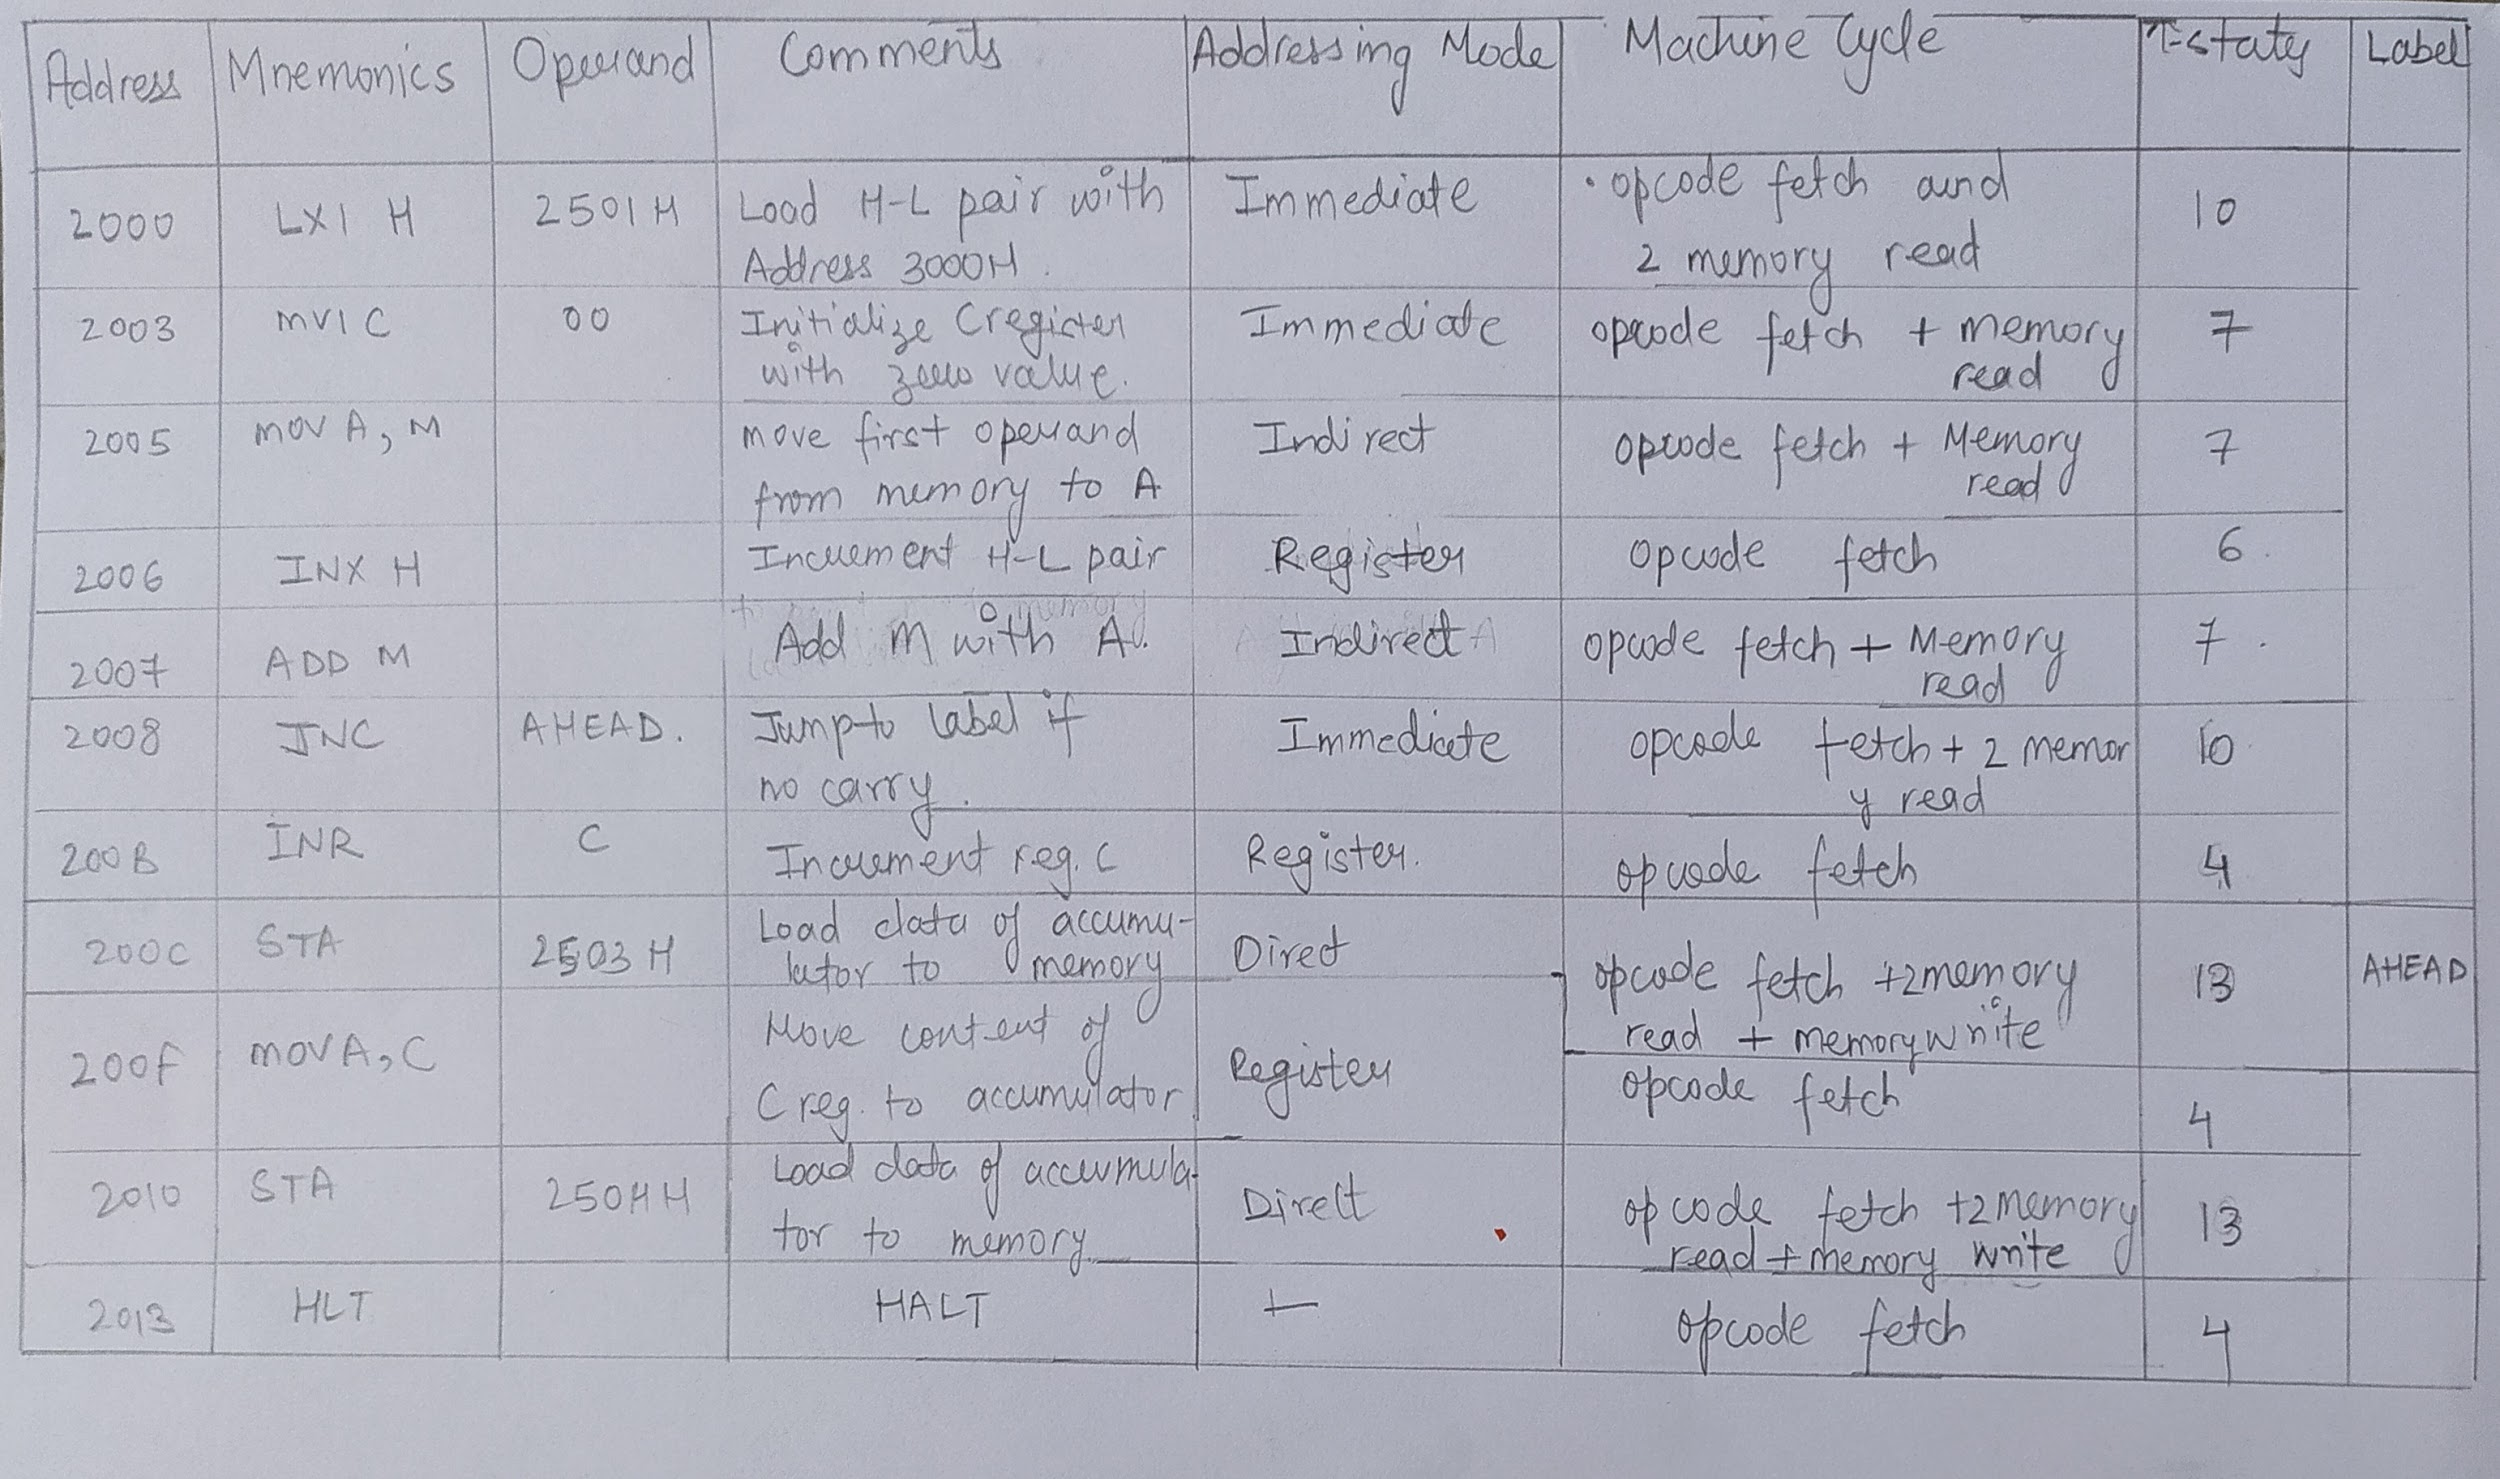
\includegraphics[width=6.5in,height=3.84722in]{media/image4.jpg}

\textbf{{[}Output:{]}}

2501- 98 H

2502- 9A H

2503- 32 H, LSBs of sum

2504- 01 H, MSBs of sum

\textbf{\href{}{RESULT}:} The sum of two 8 bit numbers in 8085 is
obtained for both the cases when

\begin{enumerate}
\def\labelenumi{\alph{enumi})}
\item
  Sum of the numbers is 8 bit
\item
  Sum of the numbers is 16 bit.
\end{enumerate}

\begin{center}\rule{0.5\linewidth}{0.5pt}\end{center}

\begin{verbatim}
Centered   Default           Right Left
 Header    Aligned         Aligned Aligned
\end{verbatim}

\begin{center}\rule{0.5\linewidth}{0.5pt}\end{center}

\begin{verbatim}
  First    row                12.0 Example of a row that
                                   spans multiple lines.

 Second    row                 5.0 Here's another one. Note
                                   the blank line between
                                   rows.
\end{verbatim}


\end{document}


